
%%%%%%%%% PROPOSAL
\noindent{\large\bf Social robot learning companions for personalized children's education}
\vspace{-4mm}   
\section{Introduction \& problem definition}
 \vspace{-3mm}   
Learning to read is one of the most important educational tasks of our schools, but in 2015, only 36\% of 4th, 34\% of 8th grade students tested on the National Assessment of Educational Progress (NAEP) reached proficiency in reading~\cite{nces2015}. Literacy skills like phonologic, alphabetic understanding, and vocabulary knowledge, delivered by quality preschool programs support the development of literacy skills in later grades and can help prevent academic failure~\cite{hart1995meaningful,paez2007dual}. Yet, only about 40\% of eligible 4 year olds attend preschool (NIEER, 2013).
I 
One of the most important factors for language skill development is sufficient exposure to a rich variety of spoken language and vocabulary \cite{asaridou2016pace}. The social context of exposure is also critical to concept development and the learning experience. Simply hearing language is not enough; children need to actively participate and be emotionally and physically engaged to maximize their learning gains~\cite{wells2000dialogic}. 

%needed to be a successful reader~\cite{wolf_2016,dehaene_2010}
When a child enters Kindergarten, they possess a unique distribution of cognitive, visual, social and linguistic skills. However, in at-risk communities it is almost impossible for a teacher to offer a curriculum that addresses the diverse cognitive and pre-literacy educational needs of each child. Young children would clearly benefit from personalized instruction that can measure and adapt to many intersecting domains of skills and abilities during the process of learning to read. 

We propose to address this challenge by developing social robot companions that can continuously assess and effectively personalize to meet individual children's diverse needs. Interactions between a child and a robot resemble the speech acts between children and adults or peers, and offer a unique opportunity to personalize social interactions to promote early literacy skills.

%Other barriers are rapidly falling: robust, affordable, and capable social robot platforms are beginning to enter the consumer market. Cloud-based infrastructure for data and computing are mature and accessible to all. Ordinary people interact daily with speech-based interfaces. Companies have recognized the importance of speech science, AI, and robotics as technologies of the future and are investing in their advancement accordingly. The time is ripe to develop the speech tools, algorithms, and models necessary to unlock the full potential of networked social robot systems to engage children and help promote early literacy skills.
\vspace{-4mm}   
\section{Innovation proposal and relation to state-of-the-art}
\vspace{-3mm}   
Social robot learning companions have great potential to augment the efforts of parents and teachers to promote learning, academic knowledge, and the wellbeing of children. Existing work with older students has shown that Intelligent Tutoring Systems (ITS) that automatically assess and adapt to student skill levels can positively impact student-learning gains~\cite{desmarais2012review}. 

%To maintain engagement and motivation during a long-term personalized interaction with younger children, a more engaging, age-appropriate, and autonomous assessment should be implemented~\cite{woolf2010building}. 

Social robots that use speech interfaces are a compelling vehicle for bringing these benefits to younger users, and while research into personalized robot tutors has gained increased attention~\cite{leyzberg2014personalizing}, the lack of reliable tools for analyzing children's speech is a major impediment to the further development and widespread deployment of truly impactful speech-based social robot tutors.

Through our research, we propose to address multiple high-impact challenges:

\subsection{Development of automatic speech recognition and spoken language understanding systems for young children's speech}
\label{section_ASR}
%\subsubsection{Automatic speech recognition for young children}
Compared to adults, children's speech is characterized by more omissions, substitutions, and mispronunciations, diversity in anatomy and developing motor skills, larger variation in spectral and temporal parameters, and larger number of disfluencies ~\cite{kennedy2017child, fainberg2016improving}. Though some tools achieve single-digit word error rate (WER) ~\cite{saon2015ibm, price2009assessment} for adult speech, there is still no robust technology for child speech with accuracy rate above 50\%; this is especially true for children younger than 7 years old.
% shorter words that make discrimination more difficult, more creative word use,

This was made clear by our analysis of the performance of several cloud-based ASR APIs on child speech, shown in Figure \ref{fig:jibo1}. We tested these APIs with a corpus of 5.5 hours of storytelling speech samples from 75 preschool and kindergarten children (ages 4-7 (5.13 $\pm$ 0.64)), collected throughout our previous projects. Results showed that no ASR API tested had less than 52\% word error rate on young children.

\begin{wrapfigure}{R}{0.35\textwidth}
\vspace{-5mm} 
  \centering
  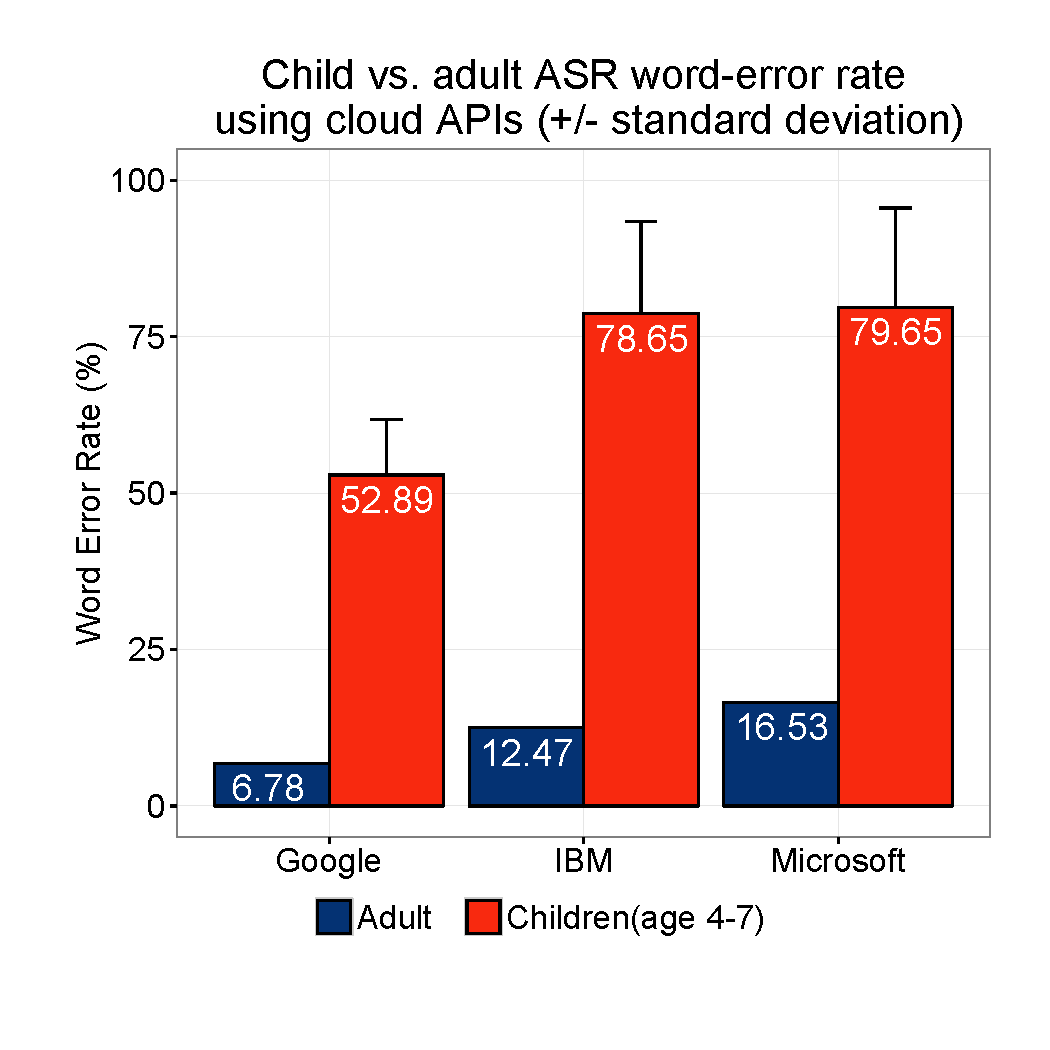
\includegraphics[width=0.35\textwidth]{fig/asr.pdf}  
  \caption{The performance of the state-of-the-art ASR tools is far from functional on child speech.}
  \vspace{-4mm}   
  \label{fig:jibo1}
\end{wrapfigure}


In preparation for this project, we have started collecting a large database of children's speech while interacting with robots in both Boston and Los Angeles Schools. We will use this data to train deep neural network (DNN) based systems for automatic speech recognition (ASR) for children's speech that are robust to age, gender, classroom noise, and disfluencies. Due to the challenges of unconstrained children's speech recognition ~\cite{fainberg2016improving}, we will restrict the domain to ASR for assessment of literacy skills, focusing on the tasks of co-reading and answering dialogic questions.

 %The goal is to develop innovative ASR algorithms for young children.
%We focus on co-reading out loud, story retell as well as dialogic scenario as: (1) The main mode of communication is speaking for our targeted age group. (2) A corpus of annotated speech from children?s reading, retelling or responding to questions from a known library of books constitutes crucially important research data to advance testing or teaching approaches, as well as the development of the theories of cognitive strategies. (3) Oral language can not only determine accuracy, but also provide cues to help diagnose understanding of vocabulary, word usage, confidence and focus.

%\subsubsection{Understanding developmental changes} 

In addition to our growing corpus of children's speech samples, we will investigate how speech and language cues develop by quantifying variation in segmental and suprasegmental properties (pitch and duration for example) in a variety of learning scenarios. To maintain ASR robustness against speaker variability and developmental changes, we will apply speaker adaptation techniques (e.g., subglottal-based normalization ~\cite{arsikere2012automatic}) to reduce spectral mismatch between training and test utterances. In addition, we will apply constraints imposed by speech production theory to model speaker variability. We also focus on noise-robustness of the ASR systems using noise robust features which retain discriminative information while suppressing information which may confuse the recognizer ~\cite{strope1998robust}; variable frame rate analysis in which we adaptively sample features according to their discriminative importance ~\cite{zhu2003non, you2004entropy}; and missing feature theory to locate and compensate for unreliable spectral components via mask estimation ~\cite{borgstrom2009missing, tan2014feature}. Finally, to ensure robustness to disfluencies and pronunciation variability, we will build acoustic models and modified dictionaries that explicitly incorporate disfluency behavior and pronunciation analysis to accurately model pronunciation variability of children from diverse linguistic backgrounds  \cite{tepperman2006pronunciation}.

%We also need to detect disfluencies in the spontaneous speech of children. Hence

%\begin{wrapfigure}{R}{0.35\textwidth}
 % \centering
 % 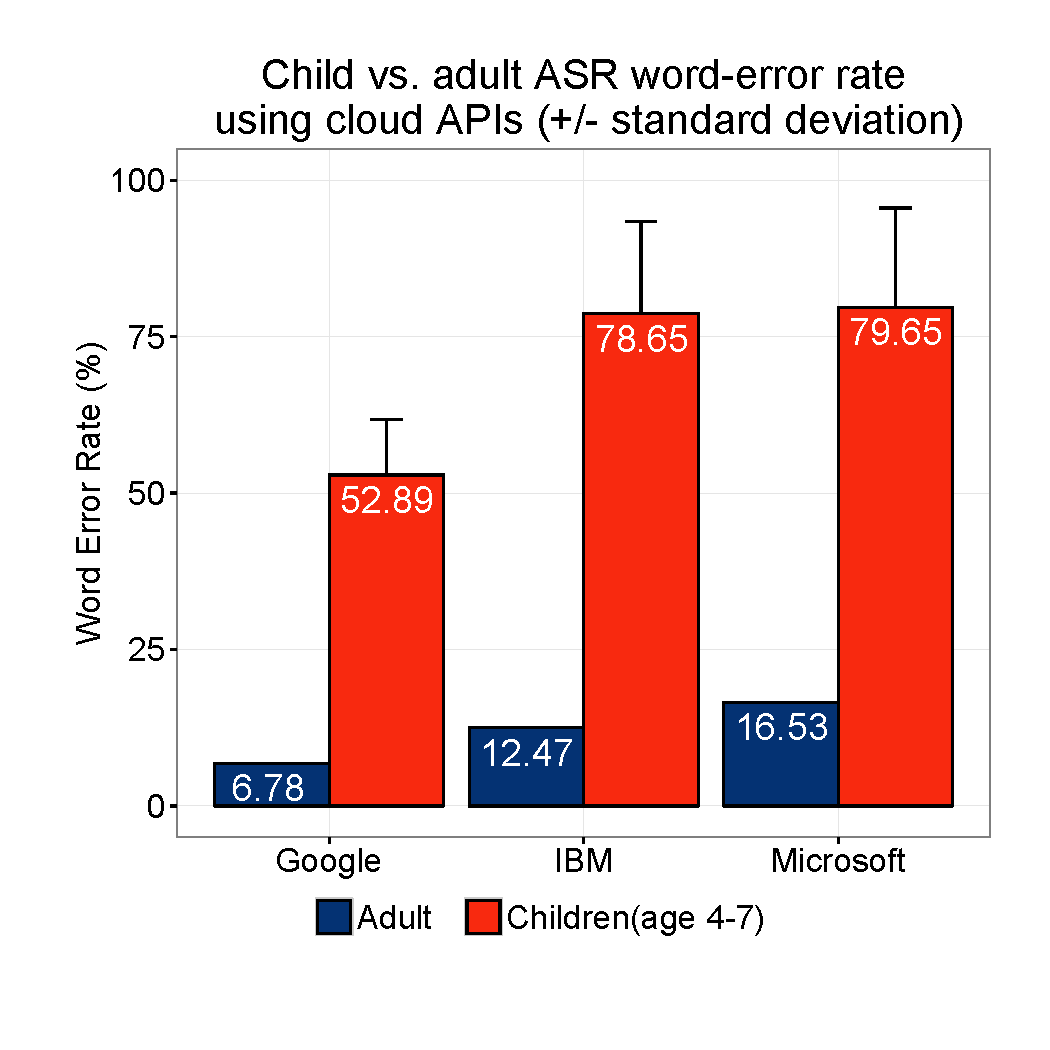
\includegraphics[width=0.35\textwidth]{fig/asr.pdf}  
 % \caption{The performance of the state-of-the-art ASR tools is far from functional on child speech.}
 % \label{fig:asr}
%\end{wrapfigure}

\subsection {Multi-modal assessment and personalization algorithms for Kindergarten age children's spoken language and early reading skills}
\label{section_assessment}

Robust child speech technologies for literacy skills will enable us to develop and deploy a new class of student models and assessment algorithms based on speech and other multi-modal data. In previous work, we showed that using affective data from facial expression to train models of children's knowledge outperformed traditional Bayesian Knowledge Tracing (BKT) models in assessing single-word reading skills~\cite{Spaulding_Gordon_Breazeal_2016}. Given our promising results with this "Affect-BKT" reading assessment algorithm for young children, we propose the following extensions to develop advanced models and algorithms that shall:

%{\bf Span to Multi-word reading tasks.} Our previous work developed Affect-BKT models that more accurately assessed student's performance on foundational, one-word reading skills. We propose to extend these results to more advanced reading skills, e.g., assessing phrases and complete sentences.

{\bf Expand beyond tactile based inputs} {\bf to spoken inputs.} Our previous work relied on a child identifying (by tapping on a touchscreen) the written form of a spoken word to assess reading ability. Our development of robust child speech technologies will enable us to incorporate speech-based data, such as spoken responses and pronunciation, enabling new interactions and multimodal models of learning.

{\bf Employ active-learning approaches} to accelerate algorithm convergence and model training. Generally speaking, assessment models and algorithms improve with additional data. But collecting additional data often requires asking more questions or prompting a child for new demonstrations of a skill. Maintaining child interest over a 20--30 minute educational interaction with an autonomous robot remains a challenge, limiting the amount of useful data from any single session. By employing an active-learning approach, the data we do collect will provide the maximum expected inferential power, allowing our models to more perform better under real-world conditions and practical data constraints.

{\bf Personalize to individual students.} In part due to data constraints, previous affect-based knowledge models were trained on data from a population of 38 children. By collecting richer, multimodal sources of real-time, real-world data and deploying the active-learning algorithms discussed above, we shall extend our work to develop personalized assessment algorithms, trained on a specific child's unique patterns of affective expression, attention, and prior knowledge.

%{\bf Incorporate hierarchical and interdependent data structures} for skill inference. Previously, our models assumed that each tracked literacy skill was mastered independently. We shall extend the Hidden Markov Model (HMM) structure of our previous Affect-BKT models to a Hierarchical Hidden Markov Model (HHMM) that captures the relationships and dependencies between skills and higher-order concepts essential to literacy development. 

\subsection {Development and evaluation of a fully autonomous, peer-like social robot system in schools and homes with effective educational activities.}

In prior work, we assessed children's oral and reading skills offline, after each interaction with a robot, which limited real-time robot behavior adaptation and curriculum personalization. Our enabling innovations of robust child ASR and improved multi-modal assessment algorithms will allow us to develop, deploy, and evaluate a completely autonomous social robot system that can adapt to children's unique educational needs over long periods of time at schools and homes. 

This robot will interact with children through a suite of educational activity apps integrating automatic speech recognition, automatic assessment and modeling of literacy (reading and linguistic) skills, and personalized content sequencing. The interaction scenario involves the social robot ``playing" educational activates with a child like a peer, using a tablet as digital interactive storybook and game surface. Through interactive storytelling and other educational activities, the social robot system will capture real-time audio, video, touch, and app states on the tablet. This data will be stored in the cloud and used to train novel computational models, assess children's reading and language performance, and adapt the content and robot's behavior in each activity to optimize children's motivation, engagement, and learning. 

%adaptation of these algorithms through innovative child ASR, collection of diverse data corpus to train and improve affect-based knowledge assessment models, and incorporating active learning methods to achieve real-time assessment and personalization. 

The ability to deliver effective, scalable, affordable, early literacy and language interventions to young children is a high impact area for the education system and parents. This proposed work extends and builds upon our teams' established track record of foundational research in the development of social robot learning companions and associated spoken interface technologies for children. By developing robust technologies for analyzing children's speech and combining these technologies with adaptive, personalized assessment algorithms, we propose to significantly advance the state-of-the-art to realize the vision of cloud-connected social robot learning companion systems that deliver effective, socially situated, and personalized spoken language education experiences for young learners.
\vspace{-4mm}   

%Relative to the current research landscape at the intersection of social robots, educational modeling, and spoken language understanding, our proposed work, while built on a firm track record of prior research, brings us into new territory with the potential for tremendous impact.
\section{One year horizon of the project}
\vspace{-3mm}   
Building on numerous past system deployments ~\cite{park2017hri-bc, gordon2016affective, westlund2017flat} we have developed and evaluated three interactive games and a shared library of grade-appropriate children's content to support multiple-month deployments. First, an interactive storybook, in which the child and the robot alternate telling versions of a given picturebook. Second, a competitive word-pronunciation game, in which the child and robot compete to win points by correctly pronouncing words, and third, a collaborative ``I Spy" game, in which the child and the robot work together to identify and pronounce words in a scene that fit a category.

\begin{figure}%{0.35\textwidth}
  \centering
  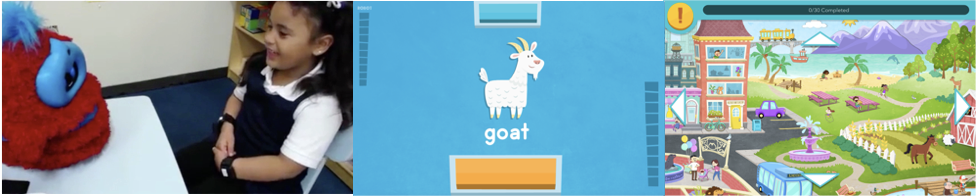
\includegraphics[width=.85\textwidth]{fig/game_screens.png}  
  \caption{3 activities designed for interactive, educational play between a robot and child to promote literacy skills.}
  \vspace{-4mm} 
  \label{fig:robots}
\end{figure}
In the first year of the project we are focusing our efforts on designing and evaluating multi-modal assessment algorithms for these games, especially in applying active and transfer learning techniques so models learned from one interaction can be used as a foundation for models in other applications or skills. During gameplay, we will also be recording audio to build up a corpus of high-quality children's speech samples for development of robust children's speech technologies.

As we collect more speech data, we will begin to develop models for children's ASR, with emphasis on: transfer learning to adapt models of adult speech to kids speech, leveraging existing speech databases, exploring model and decoding algorithm adaptation, and non-traditional feature selection.



%adding domain knowledge about speech content to model grammars and dictionary to improve accuracy,
\vspace{-4mm}   
\section{Strength of Team to Achieve Proposed Milestones}
\vspace{-3mm}
The UCLA Speech Processing and Auditory Perception Lab has an extensive history developing noise-robust speech recognition and analysis tools for children and adults.  

%\begin{wrapfigure}{R}{0.35\textwidth}
%  \centering
%  \includegraphics[width=0.35\textwidth]{fig/tega_jibo_combined.png}  
%  \caption{Proposed social robot platforms. Tega (left) is a robust research platform designed and built at MIT; Jibo (right) is a commercially-available, consumer-grade social robot platform.}
%  \label{fig:robots}
%\end{wrapfigure}

The Personal Robots Group at the MIT Media Lab has developed numerous social robot research platforms capable of sustaining engagement and interest in repeated interactions. Over the past several years, they have built extensive cloud-based infrastructure and institutional relationships to support long-term deployments of these systems in schools, hospitals, and homes. Most recently, they completed an 8 week parallel deployment of adaptive storytelling robots across 3 public schools in the Boston area.


%This proposed effort both integrates and expands our team's strong track record of foundational innovations in the development of social robot learning companion technologies that has yielded positive learning outcomes for young children in school deployments. We
